%    
%    LaTex Template: Rapport
%    Author: Chenle Li
%    Date: November 2018
%    

\documentclass{article}
\usepackage{pgfornament}
\usepackage{tikz}
\usepackage{amsmath}
\usepackage[francais]{babel}
%\usepackage{romannum}
\usepackage{hyperref}
\usepackage{color}
\usepackage{multicol}
\usepackage{titlesec}
\usepackage{amssymb}
\usepackage{amsthm}
\usepackage{fontspec}
\usepackage{parskip}
\usepackage{fourier-orns}
\setlength{\parindent}{0cm}
\usepackage{fontspec}
\setmainfont[Ligatures=TeX]{Georgia}
\setsansfont[Ligatures=TeX]{Arial}
\usepackage{blindtext}
\usepackage[margin=1in]{geometry}

\newtheorem{thm}{Th\'eor\'eme}
\newtheorem{lem}{Lemme}[thm]

\titleformat{\section}[block]{\parbox[c]{5em}{\pgfornament[width=4em]{17}}\begin{minipage}{\dimexpr\textwidth-10em\relax}\normalfont\Large\bfseries}{\thesection}{1em}{}
[{\end{minipage}\parbox[c]{5em}{\hfill\pgfornament[width=4em]{18}}}]
\titleformat*{\subsection}{\normalsize\bfseries}

\titlespacing*{\section}{0pt}{*0.5}{*0.25}

\renewcommand{\thesection}{\Roman{section}} 
\renewcommand{\thesubsection}{\thesection.\Roman{subsection}}


\title{R\'esolution Num\'erique de Equation de Schrodinger}
\author{Chenle Li \\CentraleSup\'elec, Beihang University}
\date{\today}
\begin{document}
\hrulefill\hspace{0.2cm} \floweroneleft\floweroneright \hspace{0.2cm} \hrulefill
{\let\newpage\relax\maketitle}

\tableofcontents

\newpage
\section{The Learning Problem}
\subsection{Question 1}

\noindent Which of the following problems are best suited for Machine Learning? Briefly justify your answer.

\vspace{0.5em}

\noindent {\bf (a) Classifying numbers into primes and non-primes.}\\

There is a clear definition of prime number, so there is no need to do machine learning.

\vspace{1em}

\noindent {\bf (b) Detecting potential fraud in credit card charges.}\\

To detect potential fraud in credit card charges, there is no clear rule, it depends on some not really explainable 
expertise, and so we need machine learning on this.

\vspace{1em}
\noindent {\bf (c) Determining the time it would take a falling object to hit the ground.}\\

This problem is solved with Newton's laws, so it is well defined, no need of machine learning in this.

\vspace{1em}

\noindent {\bf (d) Determining the optimal cycle for traffic lights in a busy intersection.}\\

This problem is a graph problem, solutions is quite complex, so this is well suited for machine learning.

\subsection{Question 2}

{\bf A scientist writes a computer program that automatically determines whether a newspaper article is about science policy based on the number of times the article contains the words ”science”, ”public”, ”open”, ”university”, ”government”, ”funding”, ”education”, ”justice”, ”law”. What kind of machine learning problem is the above one? Explain briefly the machine learning pipeline that you will be following to deal with this problem. [Keep your answer short; max. 10 lines]}

\vspace{1em}


It is a classification problem: determine an article is about science policy (target) from a groupe of informations (features).

Steps:
\begin{itemize}
	\item[1] Load the dataset : a dataset with a boolean label "Science Policy", and the frequency of each words in the article. 
	
	\item[2] Extract features : the frequency of each word in the article.
	
	\item[3] Model selection : Do a benchmark of classification method on the dataset.
	
	\item[4] Model training : Train the model, and get the performance like auc curve of models.

\end{itemize}


\subsection{Question 3}

Are the following machine learning problems? If yes, of what type? What are the design (data) matrix and, if appropriate, the target vector? [Keep your answer short]

\vspace{1em}

{\bf (a) Given a car owner’s manual and the price of gas at the nearest gas station, predict how much it will cost to fill up the cars tank.}\\

No.


\vspace{1em}
{\bf (b) Compute a house’s heating loads (i.e., the amount of energy that is needed to maintain the temperature) from its building plan and a civil engineer’s records of plans and heating loads for houses in the same neighborhood.}\\


Yes, knowing the heating loads of neighbors, base on seasons and house's surface (as features), we can predict the heating load of an other house.

The data matrix could be house's surface, volume, number of roms, the target vector is "heating loads"




\newpage
\section{Dimensionality Reduction}
\subsection{Question 4}

Let $M_{m\times n}$ be a data matrix ($m$ observations (i.e., data points), $n$ dimensions (i.e., features)).

\vspace{1em}

{\bf (a) Are the matrices $MM^{T}$ and $M^{T}M$ symmetric, square and real? Justify your answer.}\\

(a) Yes.
\begin{itemize}
	\item $(MM^T)^T = (M^T)^TM^T=MM^{T}$\\ symmetric proved. Same prove for $M^{T}M$.
	\item $M_{m\times n}M_{m\times n}^T=MM^T_{m\times m}$\\  $M_{m\times n}^TM_{m\times n}^=M^TM_{n \times n}$ square proved.
	\item Note $\lambda$ an eigenvalue of matrix $MM^{T}$ : \\
	$MM^{T}v=\lambda v$. \\   $ \langle MM^{T}v,MM^{T}v\rangle = v^*(MM^T)^* MM^T v = v^* (MM^T)^T MM^T v$\\ $=v^* MM^TMM^Tv=v^* \lambda^2 v =\lambda^2 \parallel v\parallel^2$\\  ${\displaystyle \lambda^2 = \frac{\langle MM^{T}v,MM^{T}v\rangle}{\parallel v\parallel^2}\geq0}$, real proved.\\ same for $M^{T}M$.
\end{itemize}


\vspace{1em}
{\bf (b) Show that the eigenvalues of $MM^{T}$ are the same as the ones of $M^{T}M$. Are their eigenvectors the same too? Justify your answer.}\\

(b)
\begin{itemize}
	\item Let $\lambda$ be an eigenvalue of $MM^T$, then $MM^Tv=\lambda v$ \\   So $M^TMM^Tv=M^T \lambda v \iff M^TM(M^Tv)=\lambda (M^T v)$. \\  $\lambda$ is an eigenvalue of $M^TM$ with the eigenvector $M^T v$

	\item No, the eigenvectors are same if $v = M^T v$ i.e. $v$ the eigenvector of $M^T$ associate eigenvalue = 1, or $M^T = id$, the 2 cases are not general.
\end{itemize}


\vspace{1em}
{\bf (c) SVD decomposes the matrix M into the product $U\Sigma V^T$, where $U$ and $V$ are orthonormal and $\Sigma$ is a diagonal matrix. Given that $M=U\Sigma V^T$, write a simplified expression of $M^{T}M$ in terms of V, V⊤ and $\Sigma$. Can we find an analogous expression for $MM^{T}$ ?}\\

(c) $M=U\Sigma V^T$. So :

\begin{itemize}
	\item $M^{T}M=(U\Sigma V^T)^T U\Sigma V^T= V \Sigma U^T U\Sigma V^T=V \Sigma^2 V^T$
	\item $MM^{T}= U\Sigma V^T (U\Sigma V^T)^T = U\Sigma V^TV\Sigma U^T = U \Sigma^2U^T $
\end{itemize}



\vspace{1em}
{\bf (d) What is the relationship (if any) between the eigenvalues of $M^{T}M$ and the singular values of $M$ ? Justify your answer.}\\


(d) $M^T$ and $M$ have the same eigenvectors for the same eigenvalues respectively.

$M^TMv=M^T(Mv)=M^T(\mu v)=\mu M^Tv=\mu (\mu v)=\mu^2 v$.

the eigenvalues of $M$ are square roots of eigenvalues of $M^TM$. 

\subsection{Question 5}

Consider 3 data points in the 2-d space: (−1, −1), (0, 0), and (1, 1).

\vspace{1em}

{\bf (a) We perform PCA on the data points. What is the first principal axis (write down the actual vector)?}

(a) $(\frac{\sqrt{2}}{2},\frac{\sqrt{2}}{2})$


\vspace{1em}
{\bf (b) If we project the data points into the 1-d subspace defined by the first principal axis, what are the coordinates of the data points in the 1-d subspace? In other words, find the first principal component of the data.}

(b)

\begin{itemize}
	\item $(-1,-1) \rightarrow -\sqrt2 $
	\item $(0,0) \rightarrow 0 $
	\item $(1,1) \rightarrow \sqrt2 $
\end{itemize}

\vspace{1em}
{\bf (c) [3 p] What is the variance of the projected data?}

(c) mean value ${\displaystyle m=\frac{\sqrt2+0+(-\sqrt2)}{3}=0}$

Variance ${\displaystyle v = \frac{(\sqrt2-0)^2 + (0-0)^2+ (-\sqrt2-0)^2}{3} = \frac{4}{3}}$




\newpage
\section{Model Evaluation and Selection}
\subsection{Question 6}

We evaluated two algorithms on a task consisting in classifying mushrooms between poisonous and edible based on some descriptors. We obtained the two following confusion matrices:

{\bf (a) Compute the accuracies of Algorithm 1 and Algorithm 2.}

(a) ${\displaystyle Acc_1 = \frac{100+97}{100+97+3}=197/200}$ 

${\displaystyle Acc_2 = \frac{100+96}{100+96+4}=196/200}$ 

$Acc_2 < Acc_1$

In term of accuracy, Algorithm 1 has higher precision than Algorithm 2.

\vspace{1em}
{\bf (b) For the task of identifying poisonous mushrooms, which algorithm is better? Explain your answer.}


(b) For this task specially, we have zero tolerance to predict a poisonous mushroom as a edible one. 

Algorithm 1 predicts 3 poisonous mushrooms as edible, 0 edible as poisonous. Algorithm 2 predicts 4 edibles mushrooms as poisonous, \textbf{0 poisonous as edible}.

So, even though the Algorithm 2 has less accuracy than Algorithm 1. We still choose the Algorithm 2.




\subsection{Question 7}

You have to implement a fraud detection system for a bank. Undetected frauds are quite costly to the bank, compared to establishing that a transaction was, in fact, not fraudulent. Which one of the following do you want to minimize? Briefly justify your answer.

{\bf (a) False positive rate}
\vspace{1em}
{\bf (b) False negative rate}
\vspace{1em}
{\bf (c) True positive rate}

False positive rate
Undetected frauds are quite costly to the bank, what we want is in fact have less cases that a fraud is predicted as not fraudulent (i.e. -1 for true class and 1 for predicted class = False positive rate).

\begin{center}
\begin{tabular}{| c | c | c |}
	\hline
	 & Fraud (-1)&No fraud (1) \\  \hline  
	Prediction Fraud (-1) &True Negative&False Negative \\   \hline  
	Prediction no Fraud (1)&False Positive&True Positive\\     
	\hline
\end{tabular}
\end{center}


\newpage
\section{Linear Regression, Logistic Regression and Feature Selection}
\subsection{Question 8}

(a) First the derivation of objective function:

\begin{equation*}
	\frac{\partial |y-X\theta|^2-\lambda|\theta|^2}{\partial x}=2\left(y-X\theta\right)^T X-2\lambda \theta^T
\end{equation*}

To minimize objective function, we need:

\begin{equation*}
	0=\frac{\partial |y-X\theta|^2-\lambda|\theta|^2}{\partial x}=2\left(X^T\left(y-X\theta\right)-\lambda \theta\right)^T=2\left(X^Ty- (1+\lambda) \theta\right)^T
\end{equation*}

So the solution is:
$$\theta=\frac{X^Ty}{1+\lambda}$$

(b) Because it reduce the complexity of model which brings generality to the model.
\subsection{Question 9}
1.Below is the graph asked in the tasks. 

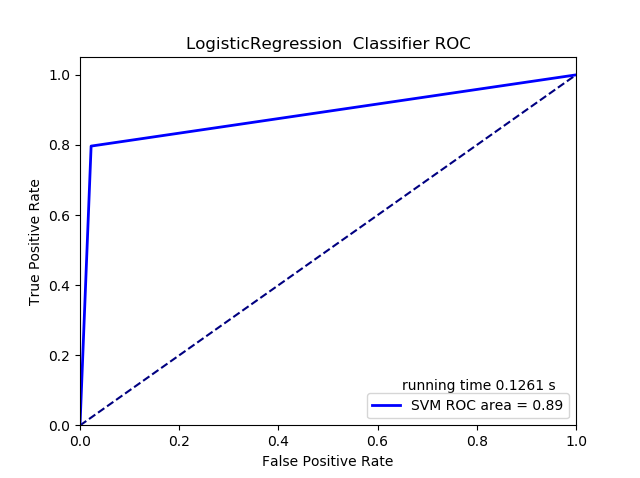
\includegraphics{MA2823MLAssignment_1/MA2823-ML-Assignment_1/Roc_Curve}

2. The model selection does improve the accuracy of the model, but it will take more time of training (\textbf{I count also the time of model selection step.})

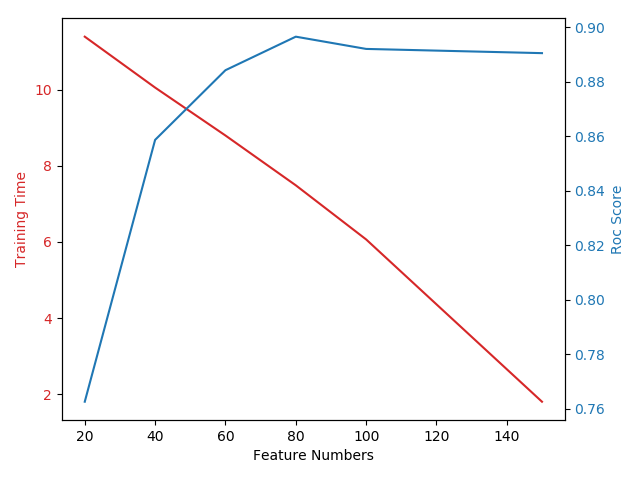
\includegraphics{MA2823MLAssignment_1/MA2823-ML-Assignment_1/Comparison}







\end{document}